\begin{figure}
  \centering
\begin{columns}
\begin{column}{0.25\textwidth}
  \begin{subfigure}[b]{\textwidth}
    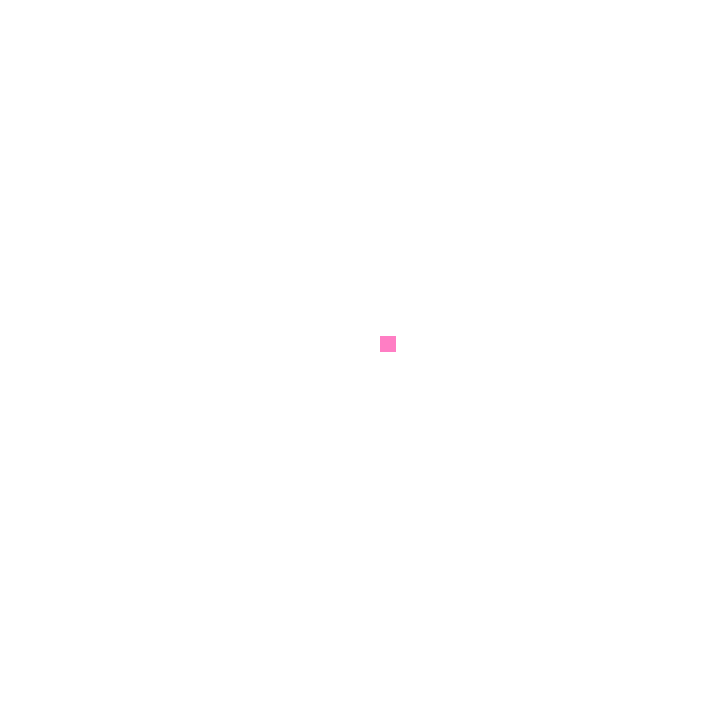
\includegraphics[width=\textwidth,trim={300 300 250 250},clip]{img/lifecycle-1}
    \caption{unicellular group}
    \label{fig:lifecycle-1}
  \end{subfigure}%
\end{column}
\begin{column}{0.05\textwidth}
  \vspace{3ex}
  
\includegraphics[width=\textwidth]{img/arrow}
\end{column}
\begin{column}{0.25\textwidth}
  \begin{subfigure}[b]{\textwidth}
    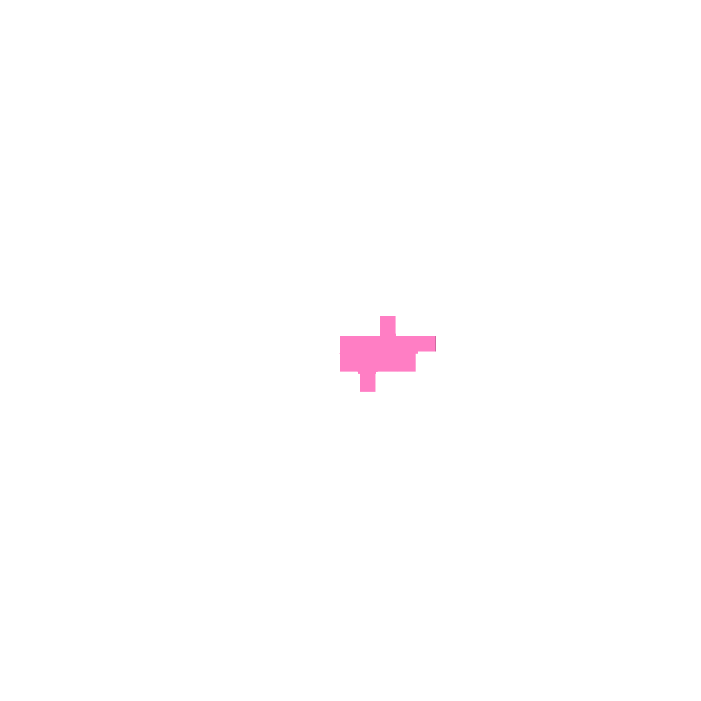
\includegraphics[width=\textwidth,trim={300 300 250 250},clip]{img/lifecycle-2}
    \caption{multicellular group}
    \label{fig:lifecycle-2}
  \end{subfigure}%
\end{column}
\begin{column}{0.05\textwidth}
  \vspace{3ex}
  
\includegraphics[width=\textwidth]{img/arrow}
\end{column}
\begin{column}{0.25\textwidth}
  \begin{subfigure}[b]{\textwidth}
    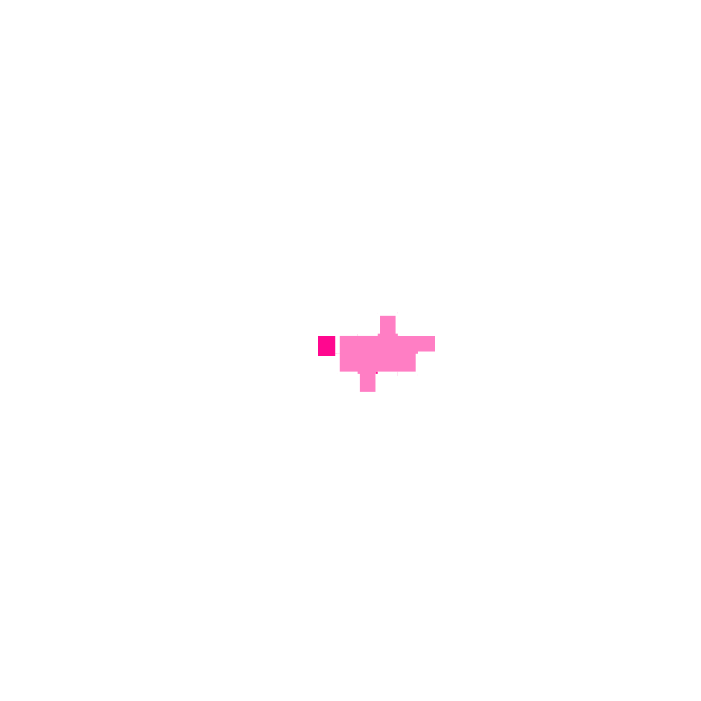
\includegraphics[width=\textwidth,trim={300 300 250 250},clip]{img/lifecycle-3}
    \caption{multicell w/ propagule}
    \label{fig:lifecycle-3}
  \end{subfigure}%
\end{column}
\begin{column}{0.2\textwidth}
\caption{
Example of nested fraternal transitions of individuality where cells (\ref{fig:cheek_cell}) unite into multicellular ants (\ref{fig:ant}), which in turn unite into ant colonies (\ref{fig:ant_bridge}).
}
\label{fig:fraternal}
\end{column}
\end{columns}
\end{figure}
